%File: formatting-instruction.tex
\documentclass[letterpaper]{article}
\usepackage{aaai}
\usepackage{times}
\usepackage{helvet}
\usepackage{courier}
\usepackage{graphicx}
\usepackage{xcolor}
\usepackage{natbib}
\bibliographystyle{aaai}
% Sudo Code packages
\usepackage[ruled, linesnumbered]{algorithm2e}

\usepackage{amsfonts}

\graphicspath{ C:/Users/Admin/OneDrive/Documents/School/CS-4080 Reinforcement Learning/ParkinglotANN/Paper/Images/ }

\frenchspacing
\setlength{\pdfpagewidth}{8.5in}
\setlength{\pdfpageheight}{11in}
\pdfinfo{
/Title (Reinforcement Learning: Parking lot)
/Author (Robert Horton)}
\setcounter{secnumdepth}{0}  
 \begin{document}

% The file aaai.sty is the style file for AAAI Press 
% proceedings, working notes, and technical reports.
%
\title{Reinforcement Learning\\ Artificial Neural Network: Valet Parking Lot }
\author{Robert Horton\\
UCCS\\
1420 Austin Bluffs Pkwy,\\
Colorado Springs, Colorado 80918\\
}
\maketitle

% ----------------------------------------------- Abstract
\begin{abstract}
\begin{quote}
With an off-policy approach the machine can be trained through different types of algorithms \& parameters to influence the rate at which the policy is found \& how optimal the policy found will be. By performing different training sessions with different types of learning agents of varying valued parameters and implementation, the machine can be expected to obtain better or worse optimal policies. Three well known off-policy learning agent implementations are \emph{Q-learning}, \emph{Double Q-Learning}, \& \emph{Self Correcting Q-Learning}. Through personal implementation \& observation of these types of algorithms \& varying parameters, the difference amongst these learning agents will be established \& the findings there of.  This study will also include the works done in other scholarly works pertaining to off-policy training methods.  For this implementation a simple parking lot environment will be rendered in which the machine can learn the optimal policy in which to perform parking a car. 
\end{quote}
\end{abstract}

% ----------------------------------------------- Introduction
\section{Introduction}

To study the different types of off-policy learning agents and their corresponding found optimal policies, an environment that is constricted to certain movements is a ideal test environment to observe \& study how these agents behave.  A simple representation of someone trying to park a car in a parking lot is a great example. Inside parking lots there are general rules that should be followed just like rules that should be followed on the road and although most parking lot can be small \& simple to navigate not all are built the same \& can be big and confusing to navigate.   Sometimes the moves the driver can make are restricted with one way lanes and other boundaries such as medians, walkways, parked cars, \& other parking spaces. Often there are big arrows and "Do Not Enter" signs to help drivers navigate the parking lot.  These different parking lots can sometimes be hard to navigate unless you are familiar with the parking lot, corresponding obstacles, \& quickest parking spots.\\
\indent Of course overtime after navigating through the same parking lot, you learn the best way to navigate the parking lot and it becomes easier \& easier to find the parkign spot you want. Sometimes the easiest thing to do when looking for a parking spot it to simply pull into to first one you see but sometimes the parking spot closest to the entrance of the store that you are going to is located on the other side of the parking lot from the entrance.  Such factors can sometimes affect the policy in which a desired parking spot is navigated to and parked in.  Ultimately, once a parking lot has become familiar and the driver knows how to get to "their" parking spot, they can usually use this information to navigate to other parking spots.  From a machine perspective this type of information can be easily represented, stored \& shared amongst different learning agents once again making it a great testing enviorment for implementing off-policy learning machines.  Further more making the testing for these types of agents and the rate at which they learn more verbose to allow for more information to be extracted and analized from different training sessions and episodes.  One problem of focus in this paper is how we can try to eliminate or at the very least to minimize the over and under estimations amongst the different off-policy learning agents.

% ----------------------------------------------- Background
\section{Background}

\indent For the testing environment that our learning agents will be trained in, the parking lot size will be represented as a six by seven array where where each state represents an element in the array. With a car we can imagine each state in the parking lot represents the space that could be occupied by the car \& the car can only occupy and move to one state as a time. The car is constrained to the outer bounds of the parking lot where the only entrance \& exit is at the bottom right corner of the parking lot. There is also the barrier in-between the parking spot in the middle row of the parking lot where the car obviously can not enter.  To keep the agent out of the barrier states \& to avoid breaking the rule of moving horizontally accross parking spots, a dictionary of illegal moves will be constructed.  Each key will be mapped to the state-action pairs that put the agent in a illegal state or move it across a parking spot illegally.  With this list when ever an action is selected to be performed by the agent, the agent can fist check to see if its a legal move or not.  If the move is illegal the reward for the what ever state would have been occupied by the action is used to calculate and update the q-table, and the agent remains in the same state \& an recursive call to select another action.  If the move is legal then the same process is done but the agent is moved to the legal state that can be occupied.\\
\indent The states that are allowed to be occupied are specific to which actions can be taken from each state. The states that the car can move through include the top two rows and bottom two rows of states.  There is also two columns, one on each of the far sides of the parking lot. The car is allowed to move through these states however the agent chooses as long as its within the boundaries and not into the middle barrier states. However the car is not allowed to move through parking spots sideways.  In other words the parking spots, labelled as P1, P2, P3, P4, P5, P6, P7, \& P8, can only be entered in by a car when the car is moving up or down.  These different actions that can be preformed from each specific state can be represented as a dictionary with key values that represent different states.  Each key value in the dictionary would then correspond to a list with four elements each element representing the action-state reward movving to that state.  This value can then update through a simple call to an "update Q-table" method that can be overwritten for each instance of different types of learning agents.  Amongst the different types of learning agents the methods in which the q-table(s) are updated \& with how often the learning agents might take exploratory steps will differ.
 Figure 1 has a picture to show a graphical representation of the parking lot.
\begin{center}
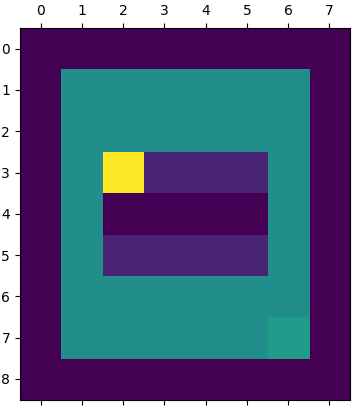
\includegraphics[scale=0.7]{parkinglot}
\end{center}

% ----------------------------------------------- Learning Agents
\section{Learning Agents}
Although the implementation will have different version of learning agents they all required a basic set of actions to perform with ultimately the same goal in mind which is to park the car in a parking spot.  Different implementations of this have been made to allow the car to park in any of the parking spots or even an given subset of the possbiel parking spots.  This was done through a simple list that maps the parking spot names, "P1", "P2", "P3", "P4", "P5", "P6", "P7", "P8", to their corresponding state.  Each agent is allowed the same range of motion including up, down, right, \& left.  These actions, even though they may be illegal from a certain state, are allowed to be chosen \& are used with the corresponding state values stored in the array that represents the parking lot.  For the purpose of this implementation setter methods for these value representation do exist but for the purpose of the main training \& this paper the values that were illegal moves are values at -100, moving through illegal states such as sides ways through parking lots states will also give a -10 return reward. Any state moved into that is a legal state will give a return reward value of -1 \& when reaching the parking spot is given a reward of 100.  The agents are also programmed to accept already initialized Q-table values from already learned values amongst other training sessions or learning agents.  Certain rules that correspond to the parking lot will also be obeyed through a mid level abstraction that allows multilevel function calls to update the learning agent state \& q-table values from the parking lot portion of the code.  This would include not driving through parking spot barriers, parking in already occupied spots, or driving though open parking spots horizontally.  When training different machines it is important for the machine to learn the best policy.  By using future rewards to calculate \& update state-action pairs \& their corresponding rewards the machine can use these values along with their set parameters \& ultimately learn the optimal policy differently.   

% ----------------------- Q-Learning 
\subsection{Q-Learning}

Although simplistic the concept of q-learning has been around for decades and many other forms, like the other implemented one in this paper, are based off the same concept.  This simple q-learning approach gives a simplistic way of evaluating state-actions \& their corresponding rewards with random actions for exploration (\cite{watkins1992q}).  From the pseudocode, a simplistic and naive off policy approach of my implementation can be described.

\begin{algorithm}[h]
 \KwData{$S=\{s_1, s_2, . \ . \  ., s_{24}, s_{25}\}$,\\
 	\quad \ \ \quad $A=\{ \leftarrow, \rightarrow, \uparrow, \downarrow \}$,\\
 	\quad \ \ \quad $Q =$72 x 4 table with arbitrary values,\\
 	\quad \ \ \quad $0 \leq \gamma \leq 1$ }
 \KwResult{Find optimal policy for Parking Car}
  initialize s\;
\While{ not in parking spot}{
 \For{episode in number of episodes}{
	ExplotOrExplore = random.choice([1, 0], weight=$\gamma$) \;
	\If{1 == ExplotOrExplore}{
		$a$ = random.choice(actions) \;
	\Else{
		$a$ = S.max($Q$) \;
		}
	}
  	 perform action $a$, observe reward $r$ \& previous state $s'$ \;
	 \tiny{$Q(s,a)\leftarrow Q(s, a)+\alpha [r+\gamma Q(s',a')-Q(s,a)]\leftarrow s'$\;
	 $s \leftarrow s' $\;}
  }
}
 \caption{Q-Learning}
\end{algorithm}
However, the learning agent that use this type of implementation can be very greedy and at times if not set with the right parameters can be very stochastic (\cite{sutton2018reinforcement}).  To combat this over estimation there have been several different methods that have been developed and deployed over the years to help remidate this under/overestimation. The basis for any q-learning based type of learning agent will consist of at least one table.  Double q-learning has two tables and will be discussed next in the paper.  At the beginning of an training session, unless a q-table with values is given to the agent, the agent assumes that all state-action rewards are zero when first intializing will set them as such.  The agent is also already implemented with the means of how to navigate the parking lot through a list of different actions it can take.  However the way the simple q-learning agent chooses to pick which actions to take is based off of a weighted random selection between taking a exploratory action or an exploited action with the highest guaranteed reward. The weighter value for each agent is set to specific values that can vary between 0.80 - 0.99. 

% ----------------------- Double Q-Learning
\subsection{Double Q-Learning}

Double q-learning like q-learning has a rather simple approach and is almost identical except that a double q-learning agent posses two different and independent q-tables.  When performing actions the learning agent either performs an exploring action or an exploited action in the same fashion with a set weighted $\gamma$ value.  The big difference is when performing either one of the two actions the agent chooses to update only one table.  This learning agent was implemented with choosing randomly between the two tables at the beginning of each action selected.  This method in many articles was shown to minimize the over estimations of selected actions and helps converge to a more optimal policy. Below is the sudo code that briefly describe how this double q-learning off policy learning agent is trained. At lines 9 we see where the agent chooses randomnly from which q-table to chose from and update.
\begin{algorithm}[tbh]
 \caption{Double Q-Learning}
   \KwData{$S=\{s_1, s_2, . \ . \  ., s_{24}, s_{25}\}$, \\
	     \quad \ \ \quad $A=\{ \leftarrow, \rightarrow, \uparrow, \downarrow \}$,\\
	     \quad \ \ \quad $Q_1 = $72 x 4 table with arbitrary values, \\
	     \quad \ \ \quad $Q_2 = $72 x 4 table with arbitrary values, \\
                \quad \ \ \quad $0 \leq \gamma \leq 1$ }

   \KwResult{Find optimal policy for Parking Car}
    initialize s\;
\While{ not in parking spot}{
   i = 0 \;
   \For{episode in number of episodes}{
	ExplotOrExplore = random.choice([1, 0], weight=$\gamma$) \;
	Q1OrQ2 = random.choice([$Q_1$, $Q_2$]\;
	\If{ExplotOrExplore == 1}{
		$a$ = random.choice(actions) \;
	\ElseIf{ExplotOrExplore == 1}{
		$a$ = S.max($Q_1$) \;
	\Else{
		$a$ = S.max($Q_2$) \;
		}
	}
  }
}
	i = Q1OrQ2 + 1\;
   	Perform action $a$, observe reward $r$ \& previous state $s'$ \;
	\tiny{$Q_i(s,a)\leftarrow Q_i(s, a)+\alpha [r+\gamma Q_i(s',a')-Q_i(s,a)]\leftarrow s'$\;
	$s \leftarrow s' $\;}
 }
\end{algorithm}
Even though double q-learning does benefit from the efficiency and simplistic off-policy approach, that it does it through various sources, one being Hasselt's paper, \textit{Double Q-Learning: Multi-agent and Adaptive Computation Group Centrum Wiskunde \& Informatica}, we see that the double q-learning approach reveals new problems .  In their paper they mention how such approaches like the one provided above do in fact help minimize the over estimations in-between steps in an episode but in fact will often underestimate.   A brief example of roulette in the paper reinforces these findings (\cite{hasselt2010double}).

% ----------------------- Self Correcting Q-Learning
\subsection{Self Correcting Q-Learning}
One such algorithm that has been suggested to overcome this underestimation is called self correcting q-learning.  This solution offers an alternative method to help avoid both the overestimation \& the underestimation that the double q-learning agent yeilds.  This type of learning agent is also different because is also involves a new parameter $\beta$ that will tune in on the optimal policy with this constant value as the bias correlation used in-between steps (\cite{zhu2021selfcorrecting}).  Through self correcting q-learning we still use the conceptual ideas of single and double estimators to help eliminate or minimize the over estimations but with an approach of updating previous state-action weighted rewards within the q-table.  These updates are made at the end of an action and once a reward is received.  Below is an example of how the code was written in sudo code. Compared to the alternatives previously discussed we see that this agent has the added parameter, $\beta$.  The steps with in the episodes is denoted as $n$  to help keep track of which steps are being back referenced to. Essentially this process can make also calculate weights in-between states that are directly related but through a set of greedy steps.  

\begin{algorithm}[h]
 \KwData{$S=\{s_1, s_2, . \ . \  ., s_{24}, s_{25}\}$,\\
 \quad \ \ \quad $A=\{ \leftarrow, \rightarrow, \uparrow, \downarrow \}$,\\
 \quad \ \ \quad $Q =$ table with arbitrary values,\\
 \quad \ \ \quad $0 \leq \gamma \leq 1$, \\
\quad  \ \ \quad $\beta \ge 1$ }
 \KwResult{Find optimal policy for Parking Car}
  initialize s\;
\While{ not in parking spot}{
 \For{episode in number of episodes}{
	ExplotOrExplore = random.choice([1, 0], weight=$\gamma$) \;
	\If{1 == ExplotOrExplore}{
		$a$ = random.choice(actions) \;
	\Else{
		$a$ = S.max($Q$) \;
		}
	}
  	  perform action $a$, observe reward $r$, previous state \& previous state $s'$ \;
	  \small{$Q^{\beta}_{n}(s',a) = Q_{n}(s', a)- \beta [Q_{n}(s',a)-Q_{n-1}(s',a)]$\; 	  
	  $MaxVal_{\beta} = max(Q^{\beta}_{n}(s',a))$ \; 
	  $Q_{n+1}(s, a) = Q_{n}(s, a) + MaxVal_{n}(s, a)[r + \gamma Q_{n}(s', MaxVal_{\beta})-Q_{n}(s,a)]$ \;
	  $s \leftarrow s' $\; }
  }
}
 \caption{Self Correcting Q-Learning}
\end{algorithm}

% ----------------------------------------------- Analysis
\section{Analysis}

It was observed and recorded that after several different attempts of learning the best policy with the different types of off-policy q-learning agents, that when given a $\gamma$ value of 0.8 or less that the optimal solution would very rarely be found.  Although the episodes would be more consistent the learning of the best policy would not be achieved, however when changing the value of $\gamma$ that agent would appear to more likely learn the optimal policy which would be up the right side of the parking lot, turning to the left after passing the second row or parking spots, and then pulling into the target parking space, ("P1").  When given a lower value for $\gamma$ the episodes would result in lots of random action choices resulting in randomly higher and low move episodes.  With the $\gamma$ set to a higher value, we can see the learning agent converge on what it thinks is the optimal policy from taking greedy actions. In this specific case, the agent somtimes will start to learn that going left and then up the far most left side of the parking lot is the best route when really it is the longer route with 12 moves.  The optimal path is going up the right side which results in 10 moves. 
From figure 2 we can see the amount of moves graphed on the y-axis with the corresponding training episode on the x-axis. The graph to the left had a $\gamma $ value or 0.9 where the right graph had a $\gamma$ of 0.8. We also see that the normal 'Q-Learning Agent' seems to learn the optimal policy a lot faster.  However although hard to tell in the graph, the learning agent learned the best policy of being able to park the car in 14 moves.  

\begin{center}

Figure 2 : Different $\gamma$ values 
\end{center}

Here in figure 3, we have the information plotted as was in figure 1 but with a 'Duble Q-Learning Agent'.  By looking at the graph we see that the agent is able to converge to the optimal policy with a few random spikes \& does not seem to have huge overestimations in performing actions resulting in move moves \& longer episodes.  
\begin{center}

Figure 3 : Double Q-Learning Agent 
\end{center}
Of course this looks a lot smoother comparatively since the training session was 200 episodes instead of 100 like the training session graphs in figure 2. With the self correcting agent the agent is able to converge to the optimal policy with less frequent spikes of under estimations and needs less explicatory moves to find the optimal policy. \\
We were also able to implement a type of learning transfer by using polymorphism \& switching between learning type agents and transferring q-tables amongst the learning agent before training sessions.  By doing so we observed that the agents were able to use the optimal policy.  However, if the table transferred is basis \& has converged on a pour policy, then no better policy will likely come from that agent although the amount of moves in between episodes for the agent will not be as dramatic as observed in experimentation.  
 
% ----------------------------------------------- Conclusion
\section{Conclusion}

In conclusion we found that ultimately off-policy learning agents can be very bias and sometimes hard to train although often is trained correctly can find the optimal policy.  With normal Q-Learning agents we have agents that have high over estimations.  With these large estimations the convergence can some times start from highly incorrect policies but as we see can eventually come to a near optimal policy.  With Double Q-Learning and Self Correcting Q-Learning we learned how to control over \& under estimations.  There are many more types of q-learning out there like deep q-learning \& backwards q-learning (\cite{WANG20132184}).This paper comes to the conclusion that Self Correcting Q-Learning can be the most beneficial from these three types covered in this paper. 

% ----------------------------------------------- References 

\bibliography{ArticleTemplate}

\end{document}